\part{Software Architecture}

Before writing the code for the demos, we started by coming up with an
overall software architecture.  The purpose of this planning was to
write each node so that as other nodes are added to our software
package we do not have to spend time rewriting old code.

This section will describe the decisions we made and what we have
planned.

\section{Node Architecture}

The main document we are basing our software architecture off of is
the following:

\FloatBarrier
\begin{figure}[h]
  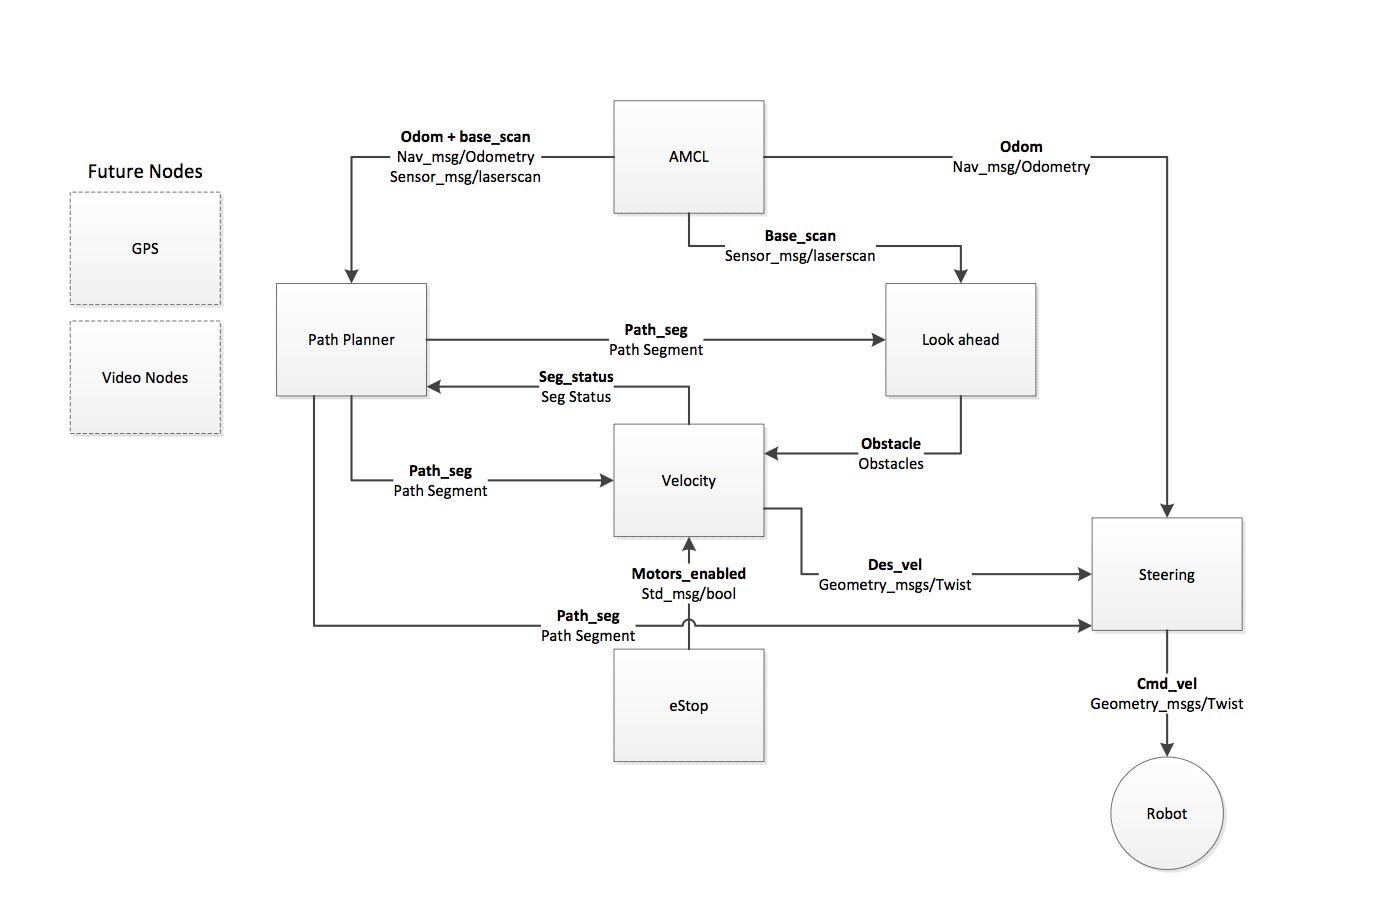
\includegraphics[width=8.0in]{software_architecture_diagram}
  \caption{Planned Software Architecture}
\end{figure}
\FloatBarrier

This figure clearly shows the different nodes we have planned, the
communication message types being passed between them, and areas of
possible future expansion.

The specifications for the nodes in the diagram and the messages being
used will be found in the rest of this section.

\section{ROS Packaging and Stacks}

We have been utilizing ROS stacks to manage our individual ROS packages.
We will try to use a single package per node. This will encourage
appropriate message passing between nodes and make sure they are not too
tightly coupled.

Another benefit is that rosmake will build packages that don't depend
on one another in parallel.  This decreases the build time by a small
amount, which is especially useful when making small changes during testing.

Stacks utilize a \texttt{stack.xml} file which contains dependencies to
be included for every package. The ROS stack will automatically build
all packages within it's root directory.

Complete documentation can be found at 
\url{http://www.ros.org/wiki/Stacks}


\section{Node Specifications}

To help guide us while writing our nodes we wrote a small
specification for each class seen in the software architecture diagram.

\subsection{Velocity Profiler}
This node is at the heart of the robot.  Nothing gets done without the
velocity profiler node running.  This node is responsible for taking
in path segments and calculating spatial trajectories.  The desired
velocities at each point along the path must obey all of the path
constraints specified by the path segment.  Path segments must be

\subsubsection{Requirements}
\begin{enumerate}
  \item Velocity Profiler must accept PathSegment messages from
    Path Planner
    \item Velocity Profiler must calculate spatial trajectories from
      the accepted PathSegment messages
      \begin{enumerate}
        \item Velocity Profiler must obey all of the path constraints
          specified in every accepted PathSegment message
         \end {enumerate}
\item Velocity Profiler must respond to Obstacle messages from Look
  Ahead
  \begin{enumerate}
    \item Velocity Profiler must stop and wait at an obstacle for a
      specified amount of time
      \item Velocity Profiler must alert Path Planner if an obstacle
        has not moved after a specified time
      \end{enumerate}
      \item Velocity Profiler must publish a desired velocity based on
        the robots current position
      \item Velocity Profiler must stop when the E-Stop is enabled
        \item Velocity Profiler must resume a plan after the E-Stop is
  disabled
  \end{enumerate}
      
  \subsection{Look Ahead}
  This node enables obstacle detection. As the name implies it is
  responsible for ``looking'' ahead for obstacles along the path.
  Currently it uses the LIDAR but other sensors such as the Kinect
  could be used to either augment or replace the LIDAR sensor data.

  \subsubsection{Requirements}
  \begin{enumerate}
  \item Look Ahead will parse the data from the LIDAR
  \item Look Ahead will detect objects within a minimum of 1 m
    \item Look Ahead will exclude obstacle detection of all objects
      outside of the planned path
      \end{enumerate}

  \subsection{Steering}
  This node is responsible for correcting the small differences
  between desired and actual heading.
  
  \subsubsection{Requirements}

  \begin{enumerate}
  \item Steering will accept paths from Path Planner
    \item Steering will correct the desired velocities from Velocity
      Profiler
    \item Steering will use a non-linear steering algorithm
      \item Steering will stop correcting the path when an obstacle is
detected
\item Steering will stop correcting the path when the E-Stop is pressed.
    \end{enumerate}

  \subsection{Path Planner}
  This node is responsible for using the robot sensors to detect the
  environment and plan a path between the robots starting position and
  the goal

  \subsubsection{Requirements}

  \begin{enumerate}
\item Path Planner will use the pre-loaded map to calculate a possible
  path
\item Path Planner will send out the calculated path in segments
\item Path Planner will respond to requests for new paths
  \item Path Planner will respond to sensory input to plan new
    segments in unknown environments
    \item Path Planner will auto-update planned paths based on
      unexpected obstacles
    \end{enumerate}

\todo[inline]{Fill in new node specifications}
  
  \subsection{Kinect}
     \subsubsection{Requirments}
     \begin{enumerate}
       \item stuff
       \end{enumerate}

  \subsection{Position Publisher}
     \subsubsection{Requirments}
     \begin{enumerate}
       \item stuff
       \end{enumerate}


     \subsection{Costmap}
     \subsubsection{Requirments}
     \begin{enumerate}
       \item stuff
       \end{enumerate}
       

  \subsection{A Star Search}
    \subsubsection{Requirments}
     \begin{enumerate}
       \item stuff
       \end{enumerate}


\todo[inline]{Check the definitions of new message specifications.}

\section{Custom Message Specifications}
\todo[inline]{Formal spec for each message that is planned. This will
  essentially be the .msg file}

\subsection{SegStatus}

Responsible for holding information about the status of a path
segment.  The message format is as follows:

\noindent {\bf bool segComplete}\\
\indent True if segment has been completed\\
\indent False if segment is still being executed\\
\\
{\bf uint64 seg\_number}\\
\indent Stores the number identifying the segment the message is
pertaining to.\\
\\
{\bf float64 distance}\\
\indent Stores the distance remaining on a segment.\\


Responsible for holding information about obstacles in the path
segments.  The message format is as follows:

\noindent {\bf bool exists}\\
\indent True when 1 or more obstacles detected in path\\
\indent False when 0 obstacles are detected in path\\
\\
{\bf float64 distance}\\
\indent The distance to the closest obstacle

\subsection{BlobDistance}
The Kinect Listener publishes the distance from the center of an image
to the center of a blob.

\noindent {\bf uint32 dist}\\
\indent Distance from the center of the blob to the center of the vision\\

\subsection{CentroidPoints}
Contains the list of coordinates of the centroids of the slices along the orange strap.
\noindent {\bf bool exists}\\
\indent \todo[inline]{What is the purpose of exists in centroid points}
\noindent {\bf geometry\_msgs/Point point}
\indent The point at which the centroid is.

\subsection{Goal}
Incrementally updates goals for the A $\ast$ search node.

\noindent{\bf bool new}\\
\indent True when a new goal is published.

\noindent{\bf bool none}\\
\indent Set to true when the robot should not change its present location.

\noindent{\bf geometry\_msgs/Point goal}\\
\indent The coordinates of the desired goal

\subsection{PathList}
A list of coordinates the A $\ast$ search publishes from the robots current position to the goal.

\noindent {\bf msg\_alpha/PathSegment[] segments}\\
\indent The coordinates of each point the robot must go to in order to reach the goal.

\subsection{PathSegment}
Path Segments that are generated by the Path Planner node.

\noindent {\bf int8 seg\_type}\\
\indent The segment type can be a line, arc, or spin, 1,2 or 3 respectivley.

\noindent {\bf bool relative}\\
\indent Set to true when the path is in the robot's coordinate frame.\\
\indent Set to false when the path is in the map's coordinate frame.

\noindent{\bf float64 seg\_length}\\
\indent The length of a path segment.

\noindent{\bf geometry\_msgs/Point ref\_point}\\
\indent The reference point of a path segment.

\noindent{\bf geometry\_msgs/Quaternion init\_tan\_angle}\\
\indent The initial tangent angle of a path segment.

\noindent{\bf float64 curvature}\\
\indent The curvature of a path segment.

\noindent{\bf geometry\_msgs/Twist max\_speeds}\\
\indent Maximum speed for a path segment.

\noindent{\bf geometry\_msgs/Twist min\_speeds}\\
\indent Minimum speed for a path segment.

\noindent{\bf float64 accel\_limit}\\
\indent Acceleration limit for a path segment 

\noindent{\bf float64 decel\_limit}\\
\indent Deceleration limit for this segment.

\subsection{PointList}
\noindent{\bf bool new}\\
\indent{\bf geometry\_msgs/Point[] points}






\section{Topics}
\todo[inline]{Short description of what each topic is publishing and why}

\subsection{des\_vel}
Velocity Profiler publishes the desired velocity based on the robot's
current point in space the current and next path segments.  This
velocity is then corrected by steering.

\subsection{cmd\_vel}
Steering publishes the final velocity to the robot's motors.  The
final velocity is a corrected version of the velocity in the des\_vel topic.

\subsection{base\_laser1\_scan and base\_scan}
base\_laser1\_scan is used on the robot\\
base\_scan is used in the simulator\\

\noindent Used to send out LIDAR data from the cRIO.

\subsection{seg\_status}
Velocity profiler publishes the status of its current segment on this
topic.  Nodes such as steering subscribe to it.

\subsection{path\_seg}
Path Publisher publishes the planned path segments to this topic.  The
published segments are used by steering, velocity\_profiler and other nodes.

\todo[inline]{Fill in functions of new topics}

\subsection{point\_list}
\subsection{goal\_point}
\subsection{path}
\subsection{obstacles}
\subsection{motors\_enabled}
